\documentclass[]{siamart}

%% ------------------------------------------------------------------
%% Code used in examples, needed to reproduce 
%% ------------------------------------------------------------------
%% Used for \set, used in an example below
\usepackage{braket,amsfonts}

%% Used in table example below
\usepackage{array,subfig}

%% Used for TIKZ example, shown in the "Figures" section below.
\usepackage{tikz}

%% Used for creating new theorems, remarks
\newsiamthm{claim}{Claim}
\newsiamremark{rem}{Remark}
\newsiamremark{ex}{Example}
\newsiamdefn{defn}{Definition}

%% Algorithm style, could alternatively use algpseudocode
\usepackage{algorithmic}

%% For figures
\usepackage{graphicx,epstopdf,subfig}

\usetikzlibrary{arrows,intersections}



%% ------------------------------------------------------------------
%% End Code used in examples, needed to reproduce 
%% ------------------------------------------------------------------


%% ------------------------------------------------------------------
%% Macros for in-document examples. These are not meant to reused for
%% SIAM journal papers.
%% ------------------------------------------------------------------
%\usepackage{environ}
\usepackage{xspace}
\usepackage{bold-extra}
\usepackage[most]{tcolorbox}
\newcommand{\BibTeX}{{\scshape Bib}\TeX\xspace}
\newcounter{example}
\colorlet{texcscolor}{blue!50!black}
\colorlet{texemcolor}{red!70!black}
\colorlet{texpreamble}{black!75}

\newcommand\bs{\symbol{'134}} % print backslash in typewriter OT1/T1
\newcommand{\preamble}[2][\small]{\textcolor{texpreamble}{#1\texttt{#2 \emph{\% <- Preamble}}}\par}

\lstdefinestyle{siamlatex}{%
  style=tcblatex,
  texcsstyle=*\color{texcscolor},
  texcsstyle=[2]\color{texemcolor},
  keywordstyle=[2]\color{texemcolor},
  moretexcs={cref,Cref},
}

\tcbset{%
  colframe=black!75!white!75,
  coltitle=white,
  colback=black!30!white!30, % left side
  colbacklower=white, % right side
  fonttitle=\bfseries,
  arc=0pt,outer arc=0pt,
  top=1pt,bottom=1pt,left=1mm,right=1mm,middle=1mm,boxsep=1mm,
  leftrule=0.3mm,rightrule=0.3mm,toprule=0.3mm,bottomrule=0.3mm,
  listing options={style=siamlatex}
}

\newtcblisting[use counter=example]{example}[2][]{%
  title={Example~\thetcbcounter: #2},#1}

\newtcbinputlisting[use counter=example]{\examplefile}[3][]{%
  title={Example~\thetcbcounter: #2},listing file={#3},#1}

\DeclareTotalTCBox{\code}{ v O{} }
{ fontupper=\ttfamily\color{texemcolor},
  nobeforeafter,
  tcbox raise base,
  colback=white,colframe=white,
  top=0pt,bottom=0pt,left=0mm,right=0mm,
  leftrule=0pt,rightrule=0pt,toprule=0mm,bottomrule=0mm,
  boxsep=0.5mm,
  #2}{#1}

\newcommand{\Comment}[2][To do]{\textcolor{red!60!yellow}{\textbf{#1:} #2}}

%% ------------------------------------------------------------------
%% End of macros for in-document examples. 
%% ------------------------------------------------------------------

\begin{document}

%% ------------------------------------------------------------------
%% HEADER
%% ------------------------------------------------------------------
\begin{tcbverbatimwrite}{\jobname_header.tex}
\title{Guide to Using SIAM's \LaTeX\ Style%
  \thanks{Acknowledgments such as funding go here.}}

\subtitle{\today} 

\author{Dianne Doe%
  \thanks{Imagination Corp., Chicago, IL (\email{ddoe@imag.com}).}%
  \and
  Paul T. Frank%
  \thanks{Department of Applied Mathematics, Fictional University, Boise, ID
    (\email{ptfrank@fictional.edu}, \email{jesmith@fictional.edu}).}
  \and
  Jane E. Smith%
  \footnotemark[3]
}

\maketitle

\end{tcbverbatimwrite}
\input{\jobname_header.tex}
%% ------------------------------------------------------------------
%% END HEADER
%% ------------------------------------------------------------------

%% ------------------------------------------------------------------
%% MARKBOTH
%% ------------------------------------------------------------------
\begin{tcbverbatimwrite}{\jobname_markboth.tex}
\pagestyle{myheadings}
\thispagestyle{plain}
\markboth{\MakeUppercase{Dianne Doe, Paul T. Frank, and Jane E. Smith}}%
{\MakeUppercase{\siampretitle\@ Guide to Using  SIAM'S \LaTeX\ Style}}
\end{tcbverbatimwrite}
\input{\jobname_markboth.tex}
%% ------------------------------------------------------------------
%% END MARKBOTH
%% ------------------------------------------------------------------



%% ------------------------------------------------------------------
%% ABSTRACT
%% ------------------------------------------------------------------
\begin{tcbverbatimwrite}{\jobname_abstract.tex}
\begin{abstract}
  Documentation is given for use of the SIAM \LaTeX\ macros.
  Instructions and suggestions for compliance with SIAM style
  standards are also included. Familiarity with standard \LaTeX\
  commands is assumed.
\end{abstract}

\begin{keywords}
  \LaTeX, \BibTeX, SIAM Journals 
\end{keywords}

\begin{AMS}
\end{AMS}
\end{tcbverbatimwrite}
\input{\jobname_abstract.tex}
%% ------------------------------------------------------------------
%% END HEADER
%% ------------------------------------------------------------------

\section{Introduction}
\label{sec:intro}

This file is documentation for the SIAM \LaTeX\ style, including how
to typeset the main document, the \BibTeX\ file, and any supplementary
material. More information
about SIAM's editorial style can be found in the style manual, available
at \url{http://www.siam.org/journals/pdf/stylemanual.pdf}.
%
The SIAM latex files can be found at
\url{http://www.siam.org/journals/auth-info.php}. The files are that
are distributed are given below. \Comment[To do]{Fix file names.}
\begin{itemize}
\item \texttt{siamart.cls} (required): Main \LaTeX\ class file.
\item \texttt{siamplain.bst} (required): Bibliographic style file for \BibTeX.
\item \texttt{docsiamart.tex}: Produces this documentation.
\item \texttt{docsiambib.bib}: Example \BibTeX\ database.
\item \texttt{docsiamsupp.tex}: Supplemental file example and documentation.
\end{itemize}
%
The outline of a SIAM \LaTeX\ article is shown in \cref{ex:outline}.

\begin{example}[label={ex:outline},listing only,%
  listing options={style=siamlatex,{morekeywords=[2]{siamart}},}]%
  {Document outline}
\documentclass{siamart}

% Packages and macros definitions go here.

\begin{document}

% Front matter goes here: title, authors, abstract, etc.
% Main body goes here.
% Appendices goes here (optional).
% Acknowledgements go here (optional).
% Bibliography goes here.

\end{document}
\end{example}

Class options can be included in the bracketed argument of the
command, separated by commas.
The \code{supplement} option specifies that the file is a supplement
and not the main document, causing changes in the appearance of the title and
numbering; see \cref{sec:supplement} for details.
By default, lines which extend past the
margin will have black boxes next to them to help authors identify
lines that they need to fix, by rewriting or inserting
breaks. Enabling the \code{final} option
turns these boxes off, so that very small margin breaks which are not
noticible will not cause boxes to be generated.
Use the \code{review} option to create line numbers before submitting
your manuscript to a SIAM journal. 


\section{Front matter}
\label{sec:front}
\Comment{We should change this to set pdftitle and pdfauthor, and then also use these in setting the page headers with markboth.}
The title and author parts are formatted using the standard
\code{\title}, \code{\author}, and \code{\maketitle} commands as
described in Lamport \cite{La86}.
%
If there is more than one author, the authors should be separated by
the \code{\and} command.  
%
The addresses and support acknowledgments are added via
\code{\thanks}. Each author's thanks should specify their address.
The support acknowledgment should be put in a thanks for the title,
unless specific support needs to be specified for individual authors,
in which case it should follow the author address.  
%
The header for this file was produced by the code in \cref{ex:header}, including an
example of a shared footnote.
%

\examplefile[label={ex:header},listing only,%
listing options={style=siamlatex,%
deletetexcs={and,thanks,title,author},%
{moretexcs=[2]{and,thanks,title,author,maketitle}}}
]{Title and authors}{\jobname_header.tex}


\Cref{ex:markboth} shows how to specify the page headings, with
the authors' names and the title (possibly shortened to fit).

\examplefile[label={ex:markboth},listing only,%
listing options={style=siamlatex,%
deletetexcs={pagestyle,thispagestyle,markboth},%
{moretexcs=[2]{pagestyle,thispagestyle,markboth}}}
]{Page headers}{\jobname_markboth.tex}

Following the author and title is the abstract, key words listing, and AMS subject
classifications, designated using the \code{abstract}, \code{keywords}, and \code{AMS}
environments. 
Authors are responsible for providing AMS numbers which can be found
on the AMS web site \cite{AMSMSC2010}. The abstract, keywords, and AMS subject classifications
for this document were specified in \cref{ex:abstract}.

\examplefile[label={ex:abstract},%
before upper={\preamble{\bs newcommand\{\bs BibTeX\}\{\{\bs scshape Bib\}\bs TeX\bs xspace\}}},
listing only,%
listing options={style=siamlatex,%
{morekeywords=[2]{abstract,keywords,AMS}}}
]{Abstract, keywords, and AMS classifications}{\jobname_abstract.tex}

\section{Cross-references and hyperlinks}

SIAM now supports cross-references and hyperlinks via the
\texttt{cleveref} and \texttt{hyperef} packages.
%
To create a cross reference, use the commands \code{\cref} (inside
sentence) and \code{\Cref} (beginning of a sentence) in place of the
object name and \code{\ref}; examples are shown in the sections below
for equations, tables, figures, sections, etc..
%
Hyperlinks are created with the \code{\href} and \code{\url} commands,
as shown in \cref{ex:href}.
SIAM has also defined the \code{\email} command, as shown in \cref{ex:header}.

\begin{example}[label={ex:href},bicolor]{Creating hyperlinks}
Click \href{http://www.siam.org}{here} to go to the SIAM homepage;
the url is \url{http://www.siam.org}.  
\end{example}

\section{Math and equations}
\label{sec:math}
Here we show some example equations, with numbering, and examples of
referencing the equations. SIAM now includes the package 
\texttt{amsmath} by default.
The SIAM \LaTeX\ class adds the following macros by default: 
\code{\const},
\code{\diag},
\code{\grad},
\code{\Range},
\code{\rank},
\code{\supp}.
%
This have the effect of rendering the item as a \texttt{mathop}.
\Cref{ex:bbm,ex:textmath,ex:smallmatrix,ex:matrices,ex:range,ex:ml,ex:aligned,ex:foo}
use many of the features of the package \code{amsmath} and examples
from \cite{MiGo04}.

\begin{example}[label={ex:bbm},bicolor,before upper={\preamble{\bs usepackage\{amsfonts\}}}]{Blackboard math}
Blackboard bold characters, such as $\mathbb{C}$ and $\mathbb{R}$,
should be created with the \texttt{amsfonts} package, although this
is not included by default.
\end{example}

\begin{example}[label={ex:textmath},bicolor]{In-line math}
The following shows normal setup of math in text: 
Let $S=[s_{ij}]$ ($1\leq i,j\leq n$) be a $(0,1,-1)$-matrix of order $n$.
\end{example}

\begin{example}[label={ex:smallmatrix},bicolor]{In-line matrix}
Matrices of no more than two rows appearing in text can be created
as shown in the next example:
$B = \bigl[ \begin{smallmatrix} B_{11} & B_{12} \\ 
  B_{21} & B_{22} \end{smallmatrix} \bigr]$.
\end{example}

\begin{example}[label={ex:matrices},bicolor]{Creating matrices}
Display matrices can be rendered using environments from \texttt{amsmath}:
\begin{equation}\label{eq:matrices}
  S=\begin{bmatrix}1&0\\0&0\end{bmatrix}
  \quad\text{and}\quad
  C=\begin{pmatrix}1&1&0\\1&1&0\\0&0&0\end{pmatrix}.
\end{equation}
Equation \cref{eq:matrices} shows some example matrices.
\end{example}

\begin{example}[label={ex:range},%
before upper={\preamble{\bs usepackage\{braket,amsfonts\}}},%
bicolor,%
listing options={style=siamlatex,%
{moretexcs=[2]{Range}}}
]{Using SIAM-defined macros}
An example of a SIAM macro:
\begin{equation}\label{eq:range}
  \Range(A) = \set{ y \in \mathbb{R}^n | y = Ax }
\end{equation}
\end{example}

\begin{example}[label={ex:ml},bicolor]{Equation split across lines}
We claim that the projection $g(U,V)$ is given by the pair of matrices:
\begin{multline} \label{eq:ml}
  g(U,V) = \biggl( \frac{R(U,V)V\Sigma^{T}U^{T} - 
      U\Sigma V^{T}R(U,V)^{T}}{2}U,\\
    \frac{R(U,V)^{T}U\Sigma V^{T}-V
      \Sigma^{T}U^{T}R(U,V)}{2}V \biggr).
\end{multline}
\end{example}

\begin{example}[label={ex:aligned},bicolor]{Subequations}
We calculate the Fr\'{e}chet derivative of $F$ as follows:
\begin{subequations}
\begin{align}
  F'(U,V)(H,K) 
  &= \langle R(U,V),H\Sigma V^{T} + U\Sigma K^{T} -
  P(H\Sigma V^{T} + U\Sigma K^{T})\rangle \label{eq:aa} \\
  &= \langle R(U,V),H\Sigma V^{T} + U\Sigma K^{T}\rangle 
  \nonumber \\
  &= \langle R(U,V)V\Sigma^{T},H\rangle + 
  \langle \Sigma^{T}U^{T}R(U,V),K^{T}\rangle. \label{eq:bb}
\end{align}
\end{subequations}
\Cref{eq:aa} is the first line, and \cref{eq:bb} is the last line.
\end{example}

\begin{example}[label={ex:foo},bicolor]{Aligned equations}
\Cref{eq:a,eq:b,eq:c} show three aligned equations.
\begin{align} 
  f &= g \label{eq:a}, \\
  f' &= g' \label{eq:b}, \quad\text{and}\\
  \mathcal{L}f &= \mathcal{L}g \label{eq:c}.
\end{align}
\end{example}

\section{Theorem-like environments}
\label{sec:thm}
SIAM uses the \texttt{ntheorem} package. Several theorem-like
environments are predefined:
\begin{itemize}
\item \code{theorem}
\item \code{lemma}
\item \code{corollary}
\item \code{definition}
\item \code{proposition}
\end{itemize}
SIAM also defines a \code{proof} environment that automatically
inserts a $\proofbox$ at the end of any proof, even if it ends in an
equation environment. \emph{Note that the document may need to be
  compiled twice for the mark to appear.}
Some of the calculus examples were adapted from \url{http://tutorial.math.lamar.edu/Classes/CalcI/MeanValueTheorem.aspx}.

% An example theorem and lemma declaration is shown in \cref{ex:theorem}.  These
% are all numbered in the same sequence and produce labels in small caps
% with an italic body. Use the command \code{\textup} to produce Roman
% type for numbers and parentheses.

\begin{example}[label=ex:theorem,bicolor,parbox=false]{Theorem}
\begin{theorem}[Mean Value Theorem]\label{thm:mvt}
  Suppose $f$ is a function that is continuous on the closed interval
  $[a,b]$.  and differentiable on the open interval $(a,b)$.
  Then there exists a number $c$ such that $a < c < b$ and
  \begin{displaymath}
    f'(c) = \frac{f(b)-f(a)}{b-a}.
  \end{displaymath}
  In other words,
  \begin{displaymath}
    f(b)-f(a) = f'(c)(b-a).
  \end{displaymath}
\end{theorem}
\end{example}

\begin{example}[label=ex:cor,bicolor,parbox=false]%
{Corollary and proof}
\begin{corollary}
  Let $f(x)$ be continuous and differentiable everywhere. If $f(x)$
  has at least two roots, then $f'(x)$ must have at least one root.
\end{corollary}
\begin{proof}
  Let $a$ and $b$ be two distinct roots of $f$.
  By \cref{thm:mvt}, there exists a number $c$ such that
  \begin{displaymath}
    f'(c) = \frac{f(b)-f(a)}{b-a} = \frac{0-0}{b-a} = 0.
  \end{displaymath}
\end{proof}
\end{example}

SIAM provides commands to create your own theorem-, definition-, and
remark-like environments:
\begin{itemize}
\item \code{newsiamthm} - Small caps header, italized body.
\item \code{newsiamdefn} - Small caps header, normal body.
\item \code{newsiamremark} - Italics header, normal body.
\end{itemize}

\begin{example}[bicolor,%
before upper={\preamble{\bs newsiamthm\{claim\}\{Claim\}}},%
parbox=false]{New theorem-like environment}
\begin{claim}\label{cl:constant}
  If $f'(x) = 0$ for all $x \in (a,b)$ then $f(x)$ is constant on $(a,b)$.
\end{claim}
\begin{proof}
  Left to reader.
\end{proof}
\end{example}

\begin{example}[bicolor,%
before upper={\preamble{\bs newsiamdefn\{defn\}\{Definition\}}},%
parbox=false]{New definition-like environment}
\begin{defn}\label{defn:sym}
  We say a matrix $A$ is \emph{symmetric} if $a_{ij} = a_{ji}$ for all $i,j$.
\end{defn}
\end{example}

\begin{example}[bicolor,%
before upper={\preamble{\bs newsiamremark\{ex\}\{Example\}}},%
parbox=false]{New remark-like environment}
\begin{ex}[Trivial note]\label{ex:a}
  Let $f(x) = 2$. Since $f'(x) = 0$ for all $x$, $f$ is constant
  everywhere.
\end{ex}
\end{example}

\begin{example}[bicolor]{References}
We can reference multiple types of objects with a single reference:
\cref{ex:a,cl:constant,thm:mvt}.
\end{example}


\section{Tables}
\label{sec:tab}

\Cref{ex:table} shows the code to generate \cref{tab:KoMa14}. This
example uses subfloats via the \texttt{subfig} package, as well as
special column options from the \texttt{array} package.

\begin{tcbverbatimwrite}{\jobname_table.tex}
\newcolumntype{R}{>{$}r<{$}}  %
\newcolumntype{V}[1]{>{[\;}*{#1}{R@{\;\;}}R<{\;]}} %
\begin{table}[htbp]
  \caption{Example table adapted from Kolda and Mayo \cite{KoMa14}.}
  \label{tab:KoMa14}
  \centering
  \subfloat[$\beta=1$]{
    \begin{tabular}{|c|R|V{3}|c|r@{\,$\pm$\,}l|} \hline
occ. & \multicolumn{1}{c|}{$\lambda$} & \multicolumn{4}{c|}{$\mathbf{x}$} & 
fevals &  \multicolumn{2}{c|}{time (sec.)}\\ \hline
 718 & 11.3476 &  0.5544 &  0.3155 &  1.2018 &  0.0977 &   45 & 0.17 & 0.06 \\ \hline 
 134 &  3.7394 &  0.2642 & -1.1056 &  0.2657 & -0.3160 &   31 & 0.12 & 0.05 \\ \hline 
 144 &  2.9979 &  1.0008 &  0.4969 & -0.0212 & -0.4817 &   31 & 0.12 & 0.05 \\ \hline 
   4 & \multicolumn{6}{c|}{\emph{--- Failed to converge ---}} & 0.21 & 0.10 \\ \hline 
 \end{tabular}}

  \subfloat[$\beta=-1$]{
    \begin{tabular}{|c|R|V{3}|c|r@{\,$\pm$\,}l|} \hline
occ. & \multicolumn{1}{c|}{$\lambda$} & \multicolumn{4}{c|}{$\mathbf{x}$} & 
fevals &  \multicolumn{2}{c|}{time (sec.)}\\ \hline
  72 & -1.1507 &  0.2291 &  0.6444 &  0.3540 & -0.8990 &   34 & 0.14 & 0.06 \\ \hline 
 150 & -3.2777 &  0.8349 & -0.7603 & -0.3532 & -0.2635 &   33 & 0.14 & 0.07 \\ \hline 
 148 & -3.5998 &  1.0486 &  0.6046 &  0.3736 &  0.3971 &   41 & 0.16 & 0.08 \\ \hline 
 624 & -6.3985 &  0.1003 &  0.1840 &  0.5305 &  1.2438 &   48 & 0.19 & 0.08 \\ \hline 
   4 & \multicolumn{6}{c|}{\emph{--- Converged to wrong solution ---}} & 0.10 & 0.11 \\ \hline 
   2 & \multicolumn{6}{c|}{\emph{--- Failed to converge ---}} & 0.23 & 0.02 \\ \hline 
 \end{tabular}}
\end{table}
\end{tcbverbatimwrite}

\examplefile[float=htpb,label={ex:table},%
before upper={\preamble[\scriptsize]{\bs usepackage\{array,subfig\}}},%
listing only, listing options={%
  style=siamlatex,basicstyle=\ttfamily\scriptsize}]%
{Example table with subtables.}{\jobname_table.tex}

\input{\jobname_table.tex}

\section{Figures}
\label{sec:fig}

\Cref{ex:fig} shows the code to generate \cref{fig:testfig}.  This
example uses the \texttt{graphicx} package for the
\code{\includegraphics} command.  SIAM requires EPS figures for final
production, but most people work in \texttt{pdflatex}. Therefore, we
recommend the package \texttt{epstopdf} to automatically convert EPS
images to PDF for inclusion in PDF documents created by
\texttt{pdflatex}.


\begin{tcbverbatimwrite}{\jobname_fig.tex}
\begin{figure}[htbp]
  \centering
  \subfloat[$\epsilon_{\max}=5$]{\label{fig:a}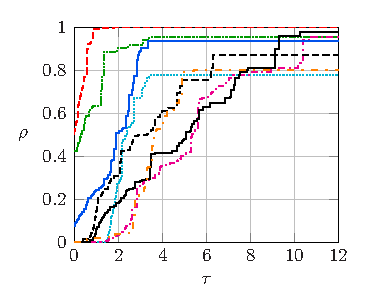
\includegraphics{lexample_fig1}}
  \subfloat[$\epsilon_{\max}=0.5$]{\label{fig:b}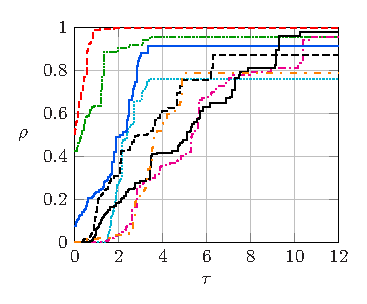
\includegraphics{lexample_fig2}}
  \caption{Example figure using external image files.}
  \label{fig:testfig}
\end{figure}
\end{tcbverbatimwrite}

\examplefile[label={ex:fig},%
before upper={\preamble[\scriptsize]{\bs usepackage\{graphicx,epstopdf,subfig\}}},%
listing only, listing options={%
  style=siamlatex,basicstyle=\ttfamily\scriptsize}]%
{Example figure with subfigures and external files}{\jobname_fig.tex}

\input{\jobname_fig.tex}

PGF is a TeX macro package for generating graphics. It is platform- and format-independent and works together with the most important TeX backend drivers, including pdftex and dvips. It comes with a user-friedly syntax layer called TikZ.
More details can be found at \url{http://sourceforge.net/projects/pgf/}, and detailed instructions are available in the manual.
\Cref{ex:tikz} shows the code to generate \cref{fig:tikz}, which uses TikZ/PGF.
This example was written by Henri Menke at
\url{http://texwelt.de/wissen/fragen/4912/skizze-zur-illustration-linearer-regression}.
\begin{tcbverbatimwrite}{\jobname_tikz.tex}
\begin{figure}[htbp]
  \centering
  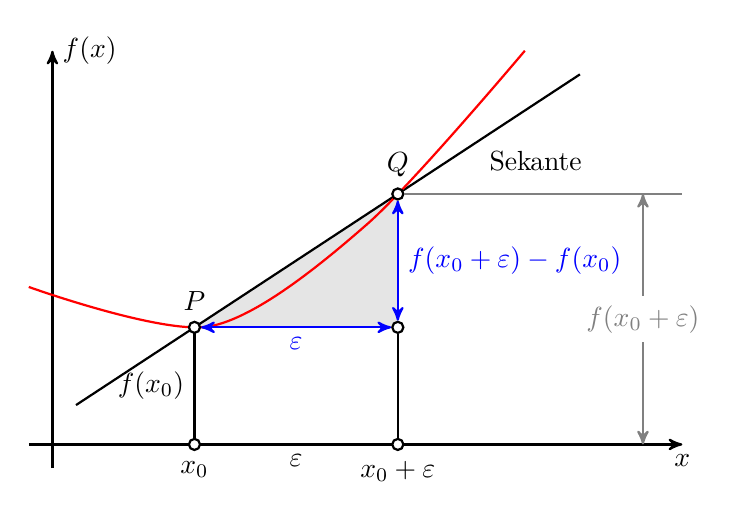
\begin{tikzpicture}[
    thick,
    >=stealth',
    dot/.style = {
      draw,
      fill = white,
      circle,
      inner sep = 0pt,
      minimum size = 4pt
    }
    ]
    \coordinate (O) at (0,0);
    \draw[->] (-0.3,0) -- (8,0) coordinate[label = {below:$x$}] (xmax);
    \draw[->] (0,-0.3) -- (0,5) coordinate[label = {right:$f(x)$}] (ymax);
    \path[name path=x] (0.3,0.5) -- (6.7,4.7);
    \path[name path=y] plot[smooth] coordinates {(-0.3,2) (2,1.5) (4,2.8) (6,5)};
    \scope[name intersections = {of = x and y, name = i}]
    \fill[gray!20] (i-1) -- (i-2 |- i-1) -- (i-2) -- cycle;
    \draw      (0.3,0.5) -- (6.7,4.7) node[pos=0.8, below right] {Sekante};
    \draw[red] plot[smooth] coordinates {(-0.3,2) (2,1.5) (4,2.8) (6,5)};
    \draw (i-1) node[dot, label = {above:$P$}] (i-1) {} -- node[left]
    {$f(x_0)$} (i-1 |- O) node[dot, label = {below:$x_0$}] {};
    \path (i-2) node[dot, label = {above:$Q$}] (i-2) {} -- (i-2 |- i-1)
    node[dot] (i-12) {};
    \draw           (i-12) -- (i-12 |- O) node[dot,
    label = {below:$x_0 + \varepsilon$}] {};
    \draw[blue, <->] (i-2) -- node[right] {$f(x_0 + \varepsilon) - f(x_0)$}
    (i-12);
    \draw[blue, <->] (i-1) -- node[below] {$\varepsilon$} (i-12);
    \path       (i-1 |- O) -- node[below] {$\varepsilon$} (i-2 |- O);
    \draw[gray]      (i-2) -- (i-2 -| xmax);
    \draw[gray, <->] ([xshift = -0.5cm]i-2 -| xmax) -- node[fill = white]
    {$f(x_0 + \varepsilon)$}  ([xshift = -0.5cm]xmax);
    \endscope
  \end{tikzpicture}
  \caption{Example TikZ figure by Henri Menke.}  
  \label{fig:tikz}
\end{figure}
\end{tcbverbatimwrite}

\examplefile[label={ex:tikz},%
before upper={\preamble[\scriptsize]{\bs usetikzlibrary\{arrows,intersections\}}},%
listing only, listing options={%
  style=siamlatex,basicstyle=\ttfamily\scriptsize}]%
{Example TikZ/PGF for platform-independent graphics.}{\jobname_tikz.tex}

\input{\jobname_tikz.tex}


\section{Algorithms}
\label{sec:algs}

\Comment{SIAM wants the algorithm caption to be small caps (which I
  have copied here), although I'm not sure why because this does not
  match the table and figures.}

\Comment{I prefer \texttt{algpseudocode} to
  \texttt{algorihmic}. Should we include neither in the header and let
  the user choose?}

\Cref{alg:buildtree} is produced by the code in \cref{ex:alg}.

\begin{tcbverbatimwrite}{\jobname_alg.tex}
\begin{algorithm}
\caption{Build tree}
\label{alg:buildtree}
\begin{algorithmic}
\STATE{Define $P:=T:=\{ \{1\},\ldots,\{d\}$\}}
\WHILE{$\#P > 1$}
\STATE{Choose $C^\prime\in\mathcal{C}_p(P)$ with $C^\prime := \operatorname{argmin}_{C\in\mathcal{C}_p(P)} \varrho(C)$}
\STATE{Find an optimal partition tree $T_{C^\prime}$ }
\STATE{Update $P := (P{\setminus} C^\prime) \cup \{ \bigcup_{t\in C^\prime} t \}$}
\STATE{Update $T := T \cup \{ \bigcup_{t\in\tau} t : \tau\in T_{C^\prime}{\setminus} \mathcal{L}(T_{C^\prime})\}$}
\ENDWHILE
\RETURN $T$
\end{algorithmic}
\end{algorithm}
\end{tcbverbatimwrite}

\examplefile[float=htpb,label={ex:alg},%
before upper={\preamble[\scriptsize]{\bs usepackage\{algorithmic\}}},%
listing only, listing options={%
  style=siamlatex,basicstyle=\ttfamily\scriptsize}]%
{Example algorithm}{\jobname_alg.tex}

\input{\jobname_alg.tex}

\section{Sections and cross-referencing}
\label{sec:sec}
Sections are denoted using standard \LaTeX\ section commands, i.e., \code{\section}, \code{\subsection}, etc. The appendices are defined the same way except that the first one is preceded by the \code{\appendix} command.
The acknowledgment section is preceeded by \code{\section*{Acknowledgments}}; it comes after any appendices and before the bibliography.

SIAM uses the \texttt{cleveref} package for cross-referencing, including
customizations to adhere to SIAM's style guidelines. 
%
The macros automatically determine the proper way to format standard
references, including the name of the reference and the hyperlink.
%
Use \code{\Cref} for a reference at the beginning of a sentence and
\code{\cref} otherwise.
%
A label for a section should always begin with \texttt{sec}.
%
\Cref{ex:secref} shows how to reference sections.


\Comment{Hyperlinks are currently black, even though they are enabled. We may want to turn on some colors for testing purposes and/or to try different options.}

\Comment{For some reason, the SIAM style does not have PDF
  bookmarks. Let's fix that.}

\Comment{Explain how to automatically reference sections in the supplement.}

\begin{example}[label={ex:secref},lefthand ratio=0.4,bicolor,sidebyside,%
listing options={style=siamlatex,basicstyle=\ttfamily\scriptsize,%
deletetexcs={cref,Cref},{moretexcs=[2]{cref,Cref}}}]
{Right and wrong ways to reference a section}
Inside a sentence\dots\\
Single: \cref{sec:intro}\\
Range: \cref{sec:intro,sec:front,%
sec:sec}\\
Multiple: \cref{sec:intro,sec:sec,%
sec:tab,sec:math,sec:thm}\\
Appendix: \cref{sec:changes}\\

Beginning of a sentence\dots\\
Single: \Cref{sec:intro}\\
Range: \Cref{sec:intro,sec:front,%
sec:sec}\\
Multiple: \Cref{sec:intro,sec:sec,%
sec:tab,sec:math,sec:thm}\\
Appendix: \Cref{sec:changes}\\


Just don't do it this way\dots\\
Section~\ref{sec:intro}  
\end{example}

\section{Supplemental material}
\label{sec:supplement}
\Comment{Explain how to do supplementary material, including \LaTeX\ files as well as multimedia.}

No appendices in supplements!

\section{Bibliography}

The SIAM \BibTeX style file, now called \texttt{siamplain.bst}, has been updated to include the new keys listed below:
\begin{itemize}
\item \code{doi}: Digital object identifier, a unique alphanumeric string
\item \code{url}: Web address, usually impermanent
\item \code{urldate}: Date that the web address was last accessed
\item \code{eprint}: Archive identifier, a unique alphanumeric string
\item \code{eprintclass}: Archive class
\item \code{archive}: Archive URL, defaults to \nolinkurl{http://arXiv.org/abs}
\item \code{archivepreprint}: Archive name, defaults to ``arXiv''.
\item \code{eid}: Article ID, if there are no page numbers
\item \code{pagetotal}: Total number of pages, for use with article ID
\end{itemize}
Every entry type has been modified to include an optional link to a
DOI, a URL, and/or an archive preprint reference.
%
Additionally, the \code{article} entry now supports an Article ID,
\code{eid}, and number of pages, \code{pagetotal}.
%
To use this, include the following code in your \LaTeX\ source code:
\code{\bibliographystyle{siamplain}}.

\subsection{DOI}

A digital object identifier (DOI) is a unique alphanumeric string that provides a persistent link to its location on the Internet. The publisher assigns a DOI when your article is published and made available electronically. Using the \code{doi} field in \BibTeX to specify it, as shown for \cite{KoMa14} in \cref{ex:article}; observe the new \code{doi} field which produces a hyperlink in the citation.
Do not include the full URL, i.e., \nolinkurl{http://dx.doi.org/} preceding the DOI.

\examplefile[label=ex:article,listing only,%
listing options={style=siamlatex,firstline=1,lastline=12,{morekeywords=[2]{doi}}}
]{Example article in \BibTeX}{docsiambib.bib}

\subsection{URL}
There is also now support for the  \code{url} field. Generally, the DOI is preferred to the URL, since the DOIs should be a permanent references. For that reason. it is good practice to specify the last date that the URL was accessed, which is specified by the optional \code{urldate} field. Reference \cite{Hi14} produced by \cref{ex:url} shows an example of using these fields.

\examplefile[label=ex:url,listing only,%
listing options={style=siamlatex,firstline=14,lastline=22,%
{morekeywords=[2]{url,urldate}}}
]{Example with the URL field in \BibTeX}{docsiambib.bib}

\subsection{Preprint servers such as arXiv}

More and more manuscripts on available on preprint servers. In fact,
SIAM's publication policy explicitly allows the final accepted version
of any article to be posted on a preprint server such as arXiv.

For an arXiv paper,
the \code{eprint} field is used to specify identifier. The optional \code{eprintclass} field specifies the class. \Cref{ex:arxiv} shows the \BibTeX for \cite{PeKoPi14}. 

\examplefile[label=ex:arxiv,listing only,%
listing options={style=siamlatex,firstline=24,lastline=32,%
{morekeywords=[2]{eprint,eprintclass}}}
]{Example arXiv reference in \BibTeX}{docsiambib.bib}

Other preprint servers are supported as well, but these require specification of the \code{archive} and \code{archiveprefix}. In this case, the target URL is formed by concatenating the \code{archive}, a forward slash (\texttt{/}), and the \code{eprint}; and the text for the hyperlink is formed by concatenating the \code{archiveprevix}, a color (:), and the \code{eprint}.
%
\Cref{ex:pubmed} shows the code to generate \cite{WoZhMeSh05}, including the preprint from PubMed.
Note that this example has both the journal citation as well as the link for the preprint.

\examplefile[label=ex:pubmed,listing only,%
listing options={style=siamlatex,firstline=34,lastline=49,%
{morekeywords=[2]{eprint,eprintclass,archive,archiveprefix}}}
]{Example PubMed reference in \BibTeX}{docsiambib.bib}

\subsection{Article ID}
Some journals use an article ID rather than page numbers. 
The field \texttt{eid} specifies the article ID. The optional field \texttt{pagetotal} can say the number
of pages in the document. An example of an article using these fields is shown in \cref{ex:eid} for citation \cite{Ne03}.

\examplefile[label=ex:eid,listing only,%
listing options={style=siamlatex,firstline=51,lastline=61,%
{morekeywords=[2]{eid,pagetotal}}}
]{Example article ID reference in \BibTeX}{docsiambib.bib}




\Comment{The new siam bib file is called \texttt{siamplain.bst}. There could also be a \texttt{siamalpha.bst} for alphabetic style references per the request of David Gleich.}


\appendix
\section{Changes}
\label{sec:changes}
The new SIAM styles includes the following significant changes as compared to older versions:
\begin{itemize}
\item Removed uppercase on title.
\end{itemize}

\section*{Acknowledgments}
Acknowledgements go here.
\Comment{Something is broken. There should not be an ``Appendix'' starting this, and the title is missing.}

\bibliographystyle{siamplain}
\bibliography{docsiambib}

\bigskip

\Comment{This files creates a bunch of extra files as it compiles. Not sure how to remove them.}

\end{document}
